\section{Theoretical Analysis}

The theoretical analysis can be subdivided in 3 parts

\subsection{DC analysis}
For the DC part, we followed a similar thought to the first code the teacher had which is: the capacitors block the current going through it! However, we chose to calculate the currents in such a way as to not divide the circuit in the same way the teacher's code did. Thus, if we define $I_{xi}$, where $x$ can be $c, e, b$ and $i$ $1, 2$, as being the currents going in the collector, emitter and base, for each of the transistors, respectively, and $I_{R1}$ and $I_{R2}$ to be the currents going through the resistors $R_1$ and $R_2$, we can then retrieve all the important information from the circuit using the matrix in \eqref{eq:dcmatrix}.

\begin{equation}
\scalemath{0.7}{
    \begin{bmatrix}
     -\beta_1 & 1 & 0 & 0 & 0 & 0 & 0 & 0\\
     0 & 0 & 0 & -\beta_2 & 1 & 0 & 0 & 0\\
     1 & 0 & 0 & 0 & 0 & 0 & -1 & 1\\
     1 & 1 & -1 & 0 & 0 & 0 & 0 & 0\\
     0 & 0 & 0 & 1 & 1 & -1 & 0 & 0\\
     0 & 0 & 0 & 0 & 0 & 0 & R_2 & R_1\\
     0 & R_c & R_e & R_c & 0 & 0 & 0 & 0\\
     0 & 0 & 0 & 0 & 0 & R_{out} & 0 & 0
    \end{bmatrix} 
    \begin{bmatrix}
        I_{b1}\\
        I_{c1}\\
        I_{e1}\\
        I_{b2}\\
        I_{c2}\\
        I_{e2}\\
        I_{R1}\\
        I_{R2}
    \end{bmatrix}
    =
    \begin{bmatrix}
        0\\
        0\\
        0\\
        0\\
        0\\
        -V_{cc}\\
        V_{cc}-V_{beon}\\
        V_{cc}-V_{beon}
    \end{bmatrix}}
\label{eq:dcmatrix}
\end{equation}
 
This then allows to for the calculation of $g_m$, $r_\pi$ and $r_o$ using the equations below.
\begin{gather}
    g_m = I_c/V_T\\
    r_\pi = \beta/g_m\\
    r_o = V_{AFN}/I_c
\end{gather}
Where each parameter is calculated for each transistor, according to the respective $\beta$ and $I_c$.
This also allows for the calculation of the output and input impedances for each stage,
\begin{gather}
    Z_{I1} = \frac{1}{\frac{1}{R_B}+\frac{r_{o1}+R_c+R_e}{(r_{o1}+R_c+R_e)(R_{\pi 1}+R_e)+g_{m1}R_er_{o1}r_{\pi 1} - R_e^2}} \\
    Z_{O1} = \frac{1}{\frac{1}{r_{o1}}+\frac{1}{R_c}}\\
    Z_{I2} = \frac{g_{m2} + g_{\pi 2} + g_{o2} + g_{e2}}{g_{\pi 2}}(g_{\pi 2} + g_{o2} + g_{e2})\\
    Z_{O2} = \frac{1}{g_{m2} + g_{\pi 2} + g_{o2} + g_{e2}}
\end{gather}

Through Octave, we get Tab.  \ref{tab:my_label}.

\begin{table}[H]
    \centering
    \begin{tabular}{c|c}
    \hline
    $Z_{I1} (\Omega)$ & $Z_{O1}(\Omega)$\\
    \hline
    $8006.605727$ & $876.533673$
    \hline
    $Z_{I2} (\Omega)$ & $Z_{O2}(\Omega)$\\
    \hline
    $6975.564760$ & $0.220603$
    \hline
    \end{tabular}
    \caption{Input and output impedances for the gain and output stages.}
    \label{tab:my_label}
\end{table}

We can also calculate immediately the total impedance through \eqref{eq:totimpd} and the value is presented in Tab. \ref{tab:totimpd}.

\begin{equation}
    Z_O = \frac{1}{g_{o2} + \frac{g_{m2}}{g_{\pi 2}}g_B + g_{e2} + g_B}
    \label{eq:totimpd}
\end{equation}

\begin{table}[H]
    \centering
    \begin{tabular}{c|c}
    \hline
    $Z_{O} (\Omega)$ & 
    $9.152525$\\
    \hline
    \end{tabular}
    \caption{Total output of the stages.}
    \label{tab:totimpd}
\end{table}

\subsection{Incremental analysis}
As for the incremental analysis, the DC voltage source $V_{cc}$ is shut down and so the nodes 0 (ground) and 6 are merged together and the transistors are approximated by the model that includes 2 capacitors, 2 resistors and a dependent voltage source (model needed in order to capture the higher cutoff frequency in the theoretical analysis). The circuit analysed in this part is presented bellow.

\begin{figure}[H]
    \centering
    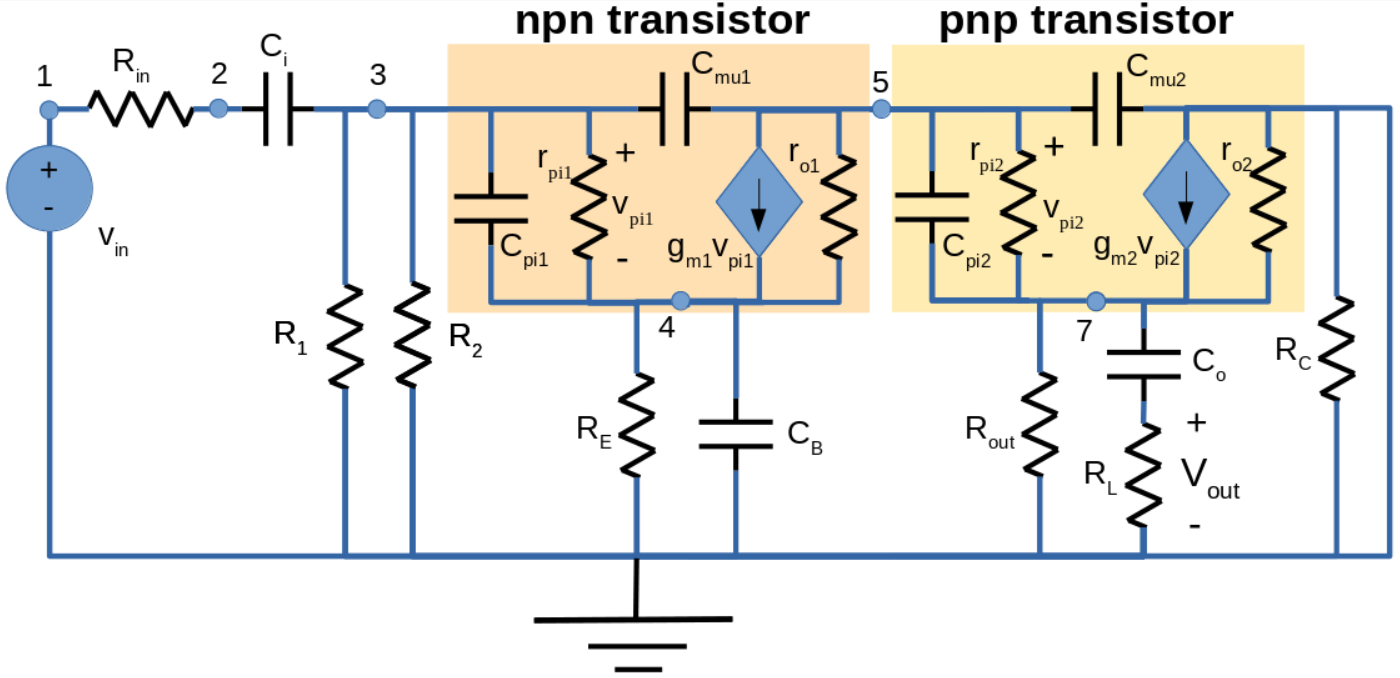
\includegraphics[width = 0.85\linewidth]{ac_analisys_circuit.pdf}
            \caption{\textit{Circuit in the incremental analysis. There is no node 6 because it was merged with ground.}}
    \label{fig:incrementalscheme}
\end{figure}

Then the nodal analysis method is applied in order to obtain in the end the output of each stage, which is $V_5$ and $V_{out}$. In order to simplify this method, $R_{in}$ and $C_i$ are merged into $Z_{in}$, disappearing node 2. Same process is applied in $R_E$ and $C_B$ that are in parallel, creating $Z_{DE}$. It is also defined $V_{0}=0$, because it's ground and $V_{1}-V_{0}=V_{in}$, which leaves only nodes 3, 4, 5, 7 and 8 for analysis.


\begin{equation}
    \begin{cases}
        \frac{V_3-V_{in}}{Z_{in}}+\frac{V_3-V_0}{R2}+\frac{V_3-V_0}{R1}+\frac{V_3-V_4}{R_{\pi1}}+(V_3-V_4)i \omega C_{\pi1}+(V_3-V_5)i \omega C_{\mu1}=0 \hspace{5mm}\text{(node 3)}\\
        \frac{V_4-V_3}{R_{\pi1}}+\frac{V_4-V_0}{Z_{DE}}+\frac{V_4-V_5}{r_{o1}}-g_{m1}(V_3-V_4)=0 \hspace{5mm}\text{(node 4)}\\
        g_{m2}(V_3-V4)+\frac{V_5-V_4}{r_{o1}}+(V_5-V_3)i \omega C_{\mu1}+\frac{V_5-V_0}{r_{C}}+(V_5-V_0)i \omega C_{\mu2}+(V_5-V_7)i \omega C_{\pi2}+\frac{V_5-V_7}{r_{\pi2}}  = 0 \hspace{15px}\text{(node 5)}\\
        (V_7-V_5)i \omega C_{\pi2}+\frac{V_7-V_5}{r_{\pi2}}+\frac{V_7-V_0}{r_{out}}+(V_7-V_8)i \omega C_o -g_{m2}(V_5-V_7)+\frac{V_7-V_0}{r_{o2}}  = 0 \hspace{15px}\text{(node 7)}\\
        (V_8-V_7)i \omega C_o+\frac{V_8-V_0}{r_{L}}  = 0 \hspace{15px}\text{(node 8)}\\
    \end{cases}
\end{equation}

Which is equivalent to the matrix form that is to be solved in Octave.

\begin{equation}
\scalemath{0.7}{
    \begin{bmatrix}
     G_{in}+G_2+G_1+G_{\pi1}+i\omega C_{\mu1} &  -G_{\pi1}      &  -i\omega C_{\mu1} &    0  &     0      \\
     -G_{\pi1}-g_{m1} & G_{\pi1}+G_{DE}+G_{o1}+g_{m1} & -G_{o1}  & 0   &  0      \\
     g_{m1}-i\omega C_{\mu1}   & g_{m1}-G_{o1}    & G_{o1}+G_C+G_{\pi2}+i\omega C_{\mu1}+i\omega C_{\mu2}  &  -G_{\pi2}-i\omega C_{\mu2}   &   0       \\
     0   & 0        & -G_{\pi2}-g_{m2}   & G_{\pi2}+G_{o2}+G_{out}+g_{m2}+i\omega C_{o} & -i\omega C_{o}      \\
     0   &  0      &  0 &  -i\omega C_{o}  &   i\omega C_{o}+G_L\\
    \end{bmatrix} 
    \begin{bmatrix}
        V_3\\
       V_4\\
        V_5\\
        V_7\\
        V_8\\
    \end{bmatrix}
    =
    \begin{bmatrix}
        V_{in}G_{in}\\
        0\\
        0\\
        0\\
        0
    \end{bmatrix}}
\label{matrix_octave_incremental}
\end{equation}